\label{sec:api}
\subsubsection{Purpose}

The back-end software component shall expose programmatic interfaces to ease the creation of modules that implement new functions (e.g. taxi reservation, taxi sharing).

The programmatic interface will consist in Java public interfaces, classes and methods.
Modules are required to use this public interface to carry out their functions, and will be limited in what they can do by this library.

The public interface shall provide safe and controlled access to the data, throwing suitable exceptions when an illegal action is attempted by a module.

\begin{figure}
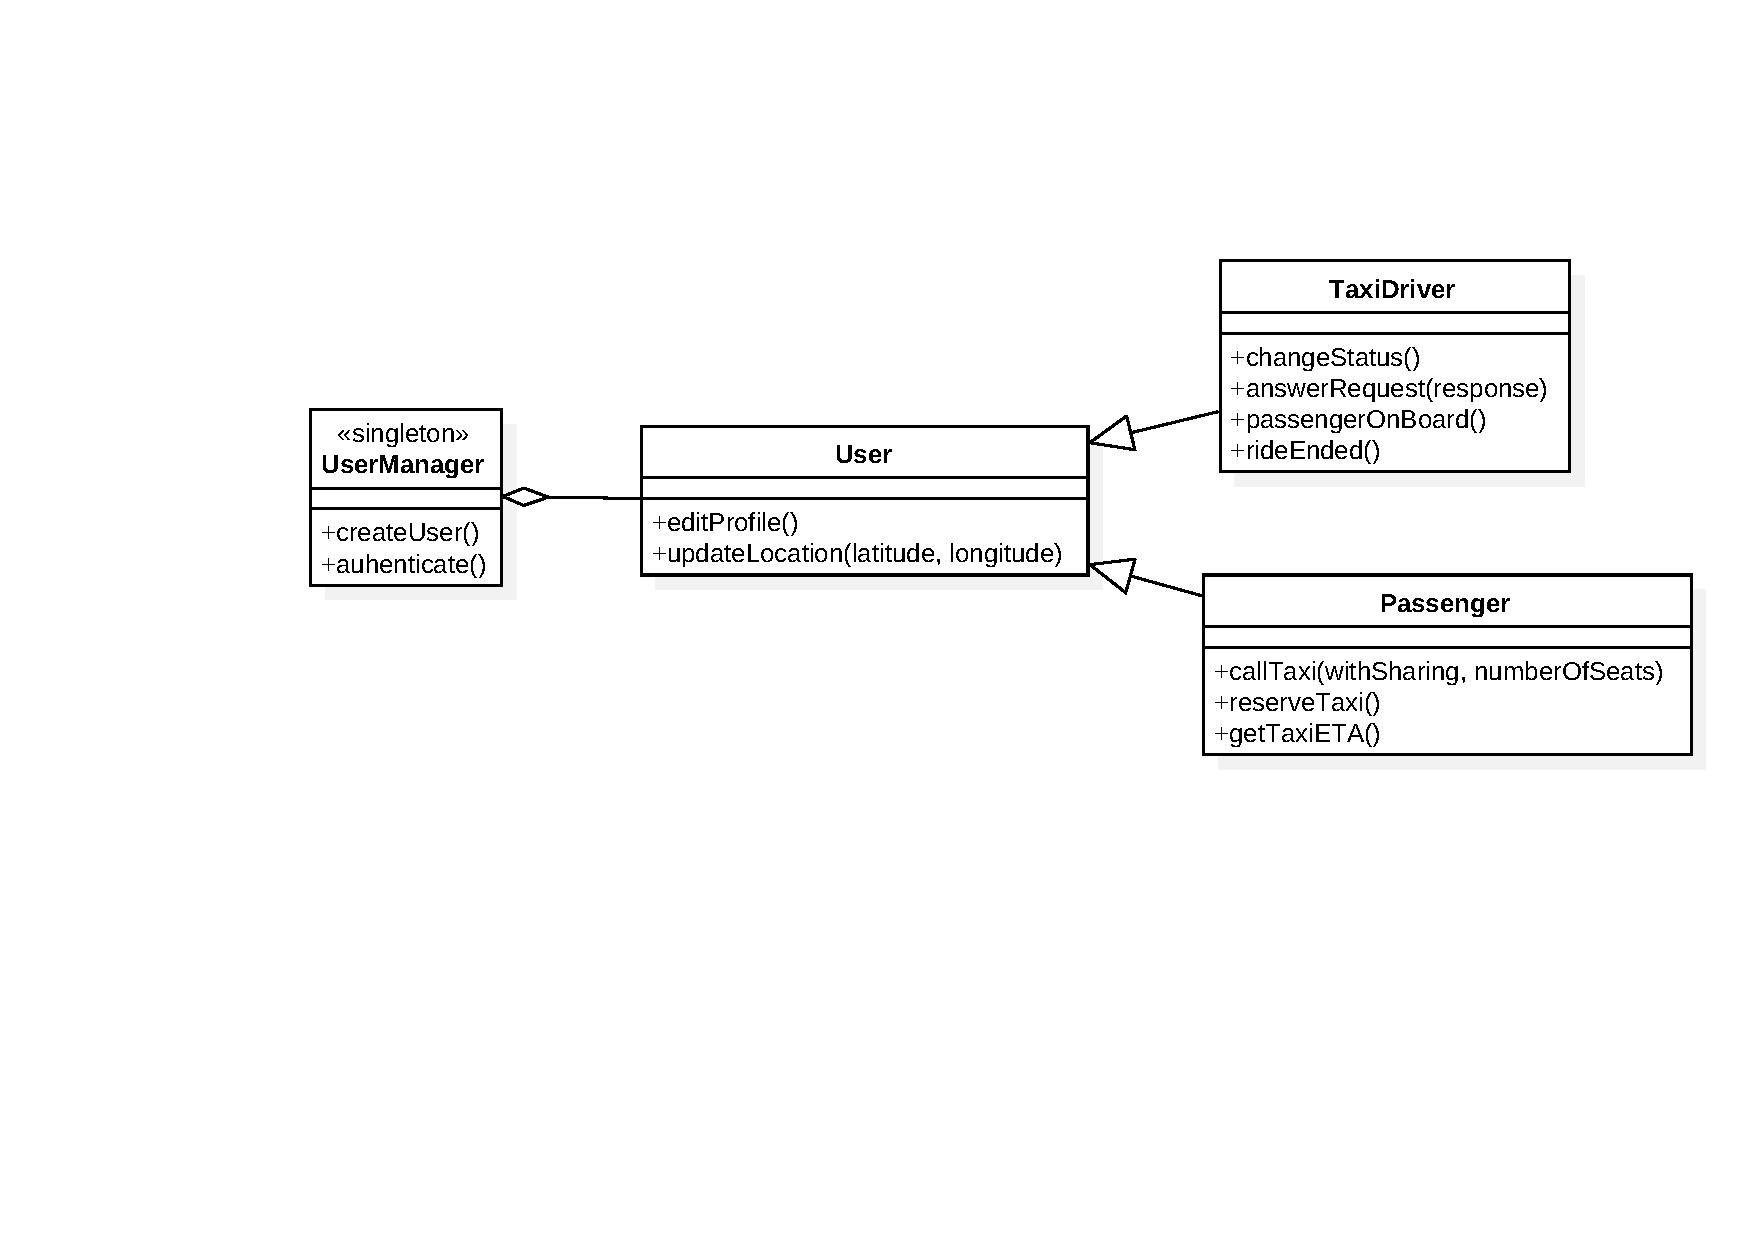
\includegraphics[width=\textwidth]{diagrams/class_programmatic.pdf}
\caption{The class diagram of the public APIs.}
\end{figure}

\subsubsection{Associated functional requirements}
\begin{enumerate}
\item Creation of a new user (taxi driver or passenger)
\begin{enumerate}
    \item The system shall have a UserManager class that allows to create new users of both passenger and taxi driver types.
    \item The class shall raise reasonable exceptions if the requirements in~\autoref{user-registration} trigger exceptions.
\end{enumerate}
\item User authentication and login
\begin{enumerate}
    \item The system must provide an interface to authenticate a user.
    \item The system must return reasonable exceptions if the login fails.
    \item If the login succeeds, the system returns to the caller a token in order for the requests to be stateful.
\end{enumerate}
\item Modification of user profile
\begin{enumerate}
    \item The system shall allow any logged user to change data in his/her profile, according to the requirements in~\autoref{user-profile}.
    \item The system shall allow any logged user to delete his/her profile, according to the requirements in~\autoref{user-profile}.
\end{enumerate}
\item Updating the location of a user
\begin{enumerate}
    \item The system shall allow external clients to update the location of the logged user.
    \item The user location must be given as latitude and longitude (GPS coordinates).
\end{enumerate}
\item Taxi availability and status handling
\begin{enumerate}
    \item The system shall provide methods that allow the taxi driver to get and change his/her status (as in~\autoref{taxi-availability}).
    \item This interface shall also accept the ``passenger on board'' and ``ride ended'' messages.
\end{enumerate}
\item Taxi call
\begin{enumerate}
    \item The system must provide a method that allows any logged in passenger to call a taxi from the current position, according to requirements in~\autoref{standard-call}.
    \item The method blocks until the request is accepted.
    \item When the request is accepted, the taxi ETA is returned.
    \item The interface must offer a method to get the updated ETA for the incoming taxi.
\end{enumerate}

\item Reservation of a taxi for a specific destination in a specific time
\begin{enumerate}
    \item The system must offer a method to let any logged in user reserve a taxi, according to requirements in~\autoref{taxi-reservation}.
    \item The user must provide the following data: initial position, destination, time of meeting.
    \item If the data is not valid (according to the same requirements), the method should raise suitable exceptions.
\end{enumerate}

\item Taxi sharing
\begin{enumerate}
	\item The system must provide a method that allows any passenger to enable sharing mode, according to requirements in~\autoref{ride-sharing}
	\item The system must allow user to provide a destination and the number of seats required when sharing mode is enabled
	\item The system must provide the user with a possibility to choose among compatible rides or a new ride
\end{enumerate}
\item Taxi driver notification
\begin{enumerate}
	\item The system must provide the taxi driver with the possibility to choose to accept or refuse an incoming request, according to requirements in~\autoref{driver-notification}
\end{enumerate}

\end{enumerate}
